\documentclass{evolang12}
\usepackage{graphicx}
\usepackage{url}
\usepackage{authblk}
\usepackage[raggedright]{sidecap}



\begin{document}


\title{What 50 million drawings can tell us about shared meaning}
\author[*1,2]{MOLLY LEWIS}
\author[1]{GARY LUPYAN}
\affil[*]{Corresponding Author: mollyllewis@gmail.com}
\affil[1]{Department of Psychology, University of Wisconsin-Madison}
\affil[2]{Computation Institute, University of Chicago}

\maketitle

A foundational assumption of linguistic communication is that conversants have similar underlying concepts \cite{brennan1996conceptual,wierzbicka2012understanding}. On this view, the ability of one person to understand another when she says ``the tree" depends on the word activating the same concept in both people. One approach to verifying this assumption is to rely on definitions, but this reasoning is circular---how can we be sure the words {\it in} our definitions are the same? Here, we investigate the assumption of shared linguistic concepts by studying concepts represented in the visual modality---drawings---and examining predictors of their variability. Specifically, we ask whether people who are geographically closer and inhabit a similar linguistic environment produce more similar drawings.

We analyzed a dataset of 50 million drawings (of mostly concrete artifacts such as ``tree") from 15 million participants (QuickDraw: quickdraw.withgoogle.com/data). Although all drawings were elicited in English, the participants spanned the globe and, we can assume, represent a wide variety of cultural and linguistic experience. Such drawings only capture a part of meaning---people know much more about trees than what they look like---and therefore offer a conservative estimate of diversity.

We quantified similarity of drawings in two ways: (1) Hausdorff Distance (HD), which quantifies image similarity as the minimum Euclidean distance between two sets of points \cite{Huttenlocher93comparingimages}; (2) the internal weights (layer FC2) for each of our drawings from a neural net model trained on ImageNet \cite{deng2009imagenet}, with similarity corresponding to the cosine distance (CD) on weights between pairs of images. 

\begin{figure}[t]
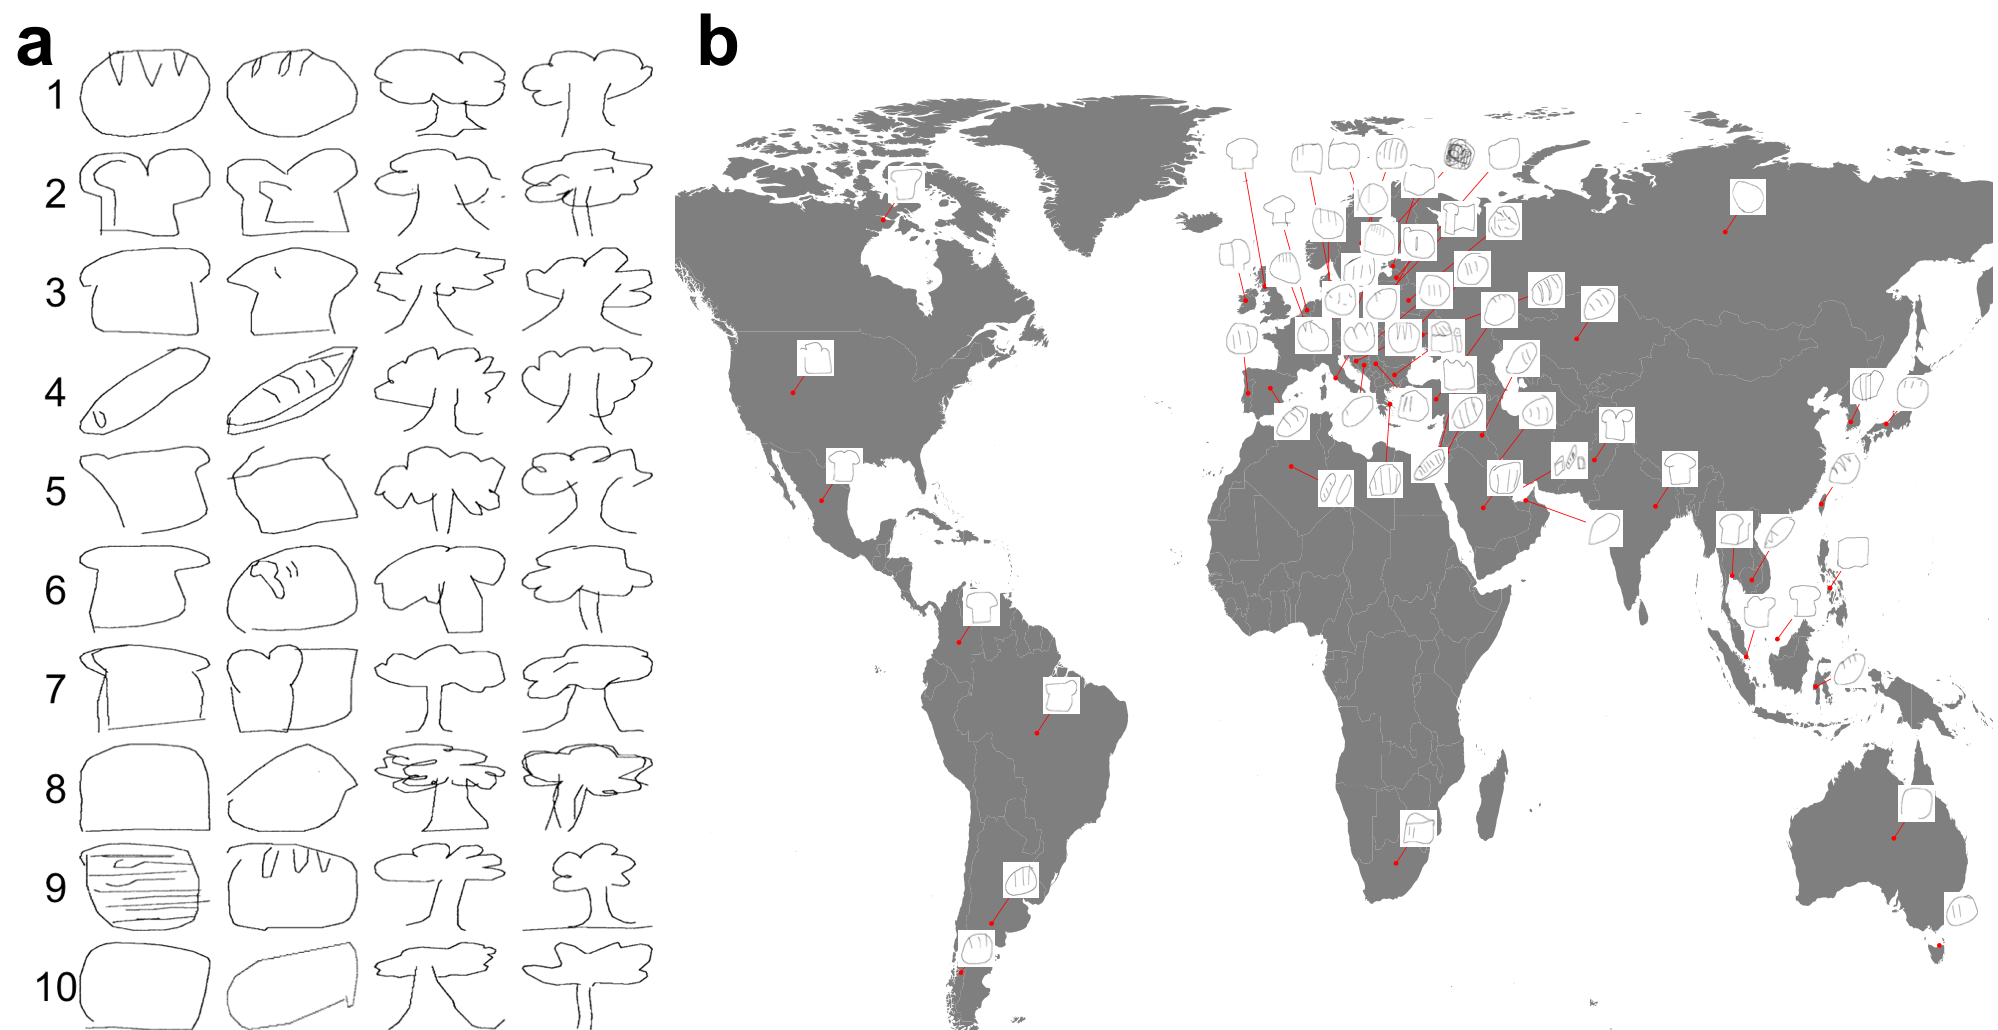
\includegraphics[width=4.55in]{full_fig3.png}
\caption{(a) Sample drawing pairs (``bread'' and ``tree'') used in the human similarity judgement experiment. Each row corresponds to a Hausdorff decile. (b) The prototypical ``bread" drawing for each country, calculated as the drawing with the smallest average pairwise distance to other drawings from the same country. \label{fig1}}
\end{figure}

Initial analysis included 1500 image pairs of two categories---``bread" and ``tree"---from participants located in 72 countries. We validated our similarity measures using human judgements. We selected 20 pairs from each HD decile for each category (Fig.\ 1a), and asked participants to rate the similarity of the objects in the drawings using a 1 (almost identical) to 7 (completely different) Likert scale. Each participant ($N$ = 100) rated 50 pairs drawings from the same category. 

Human judgements of similarity were highly correlated with HD ($r$ = .29, $p <$ .0001) as well as CD ($r$ = 0.20, $p <$ .0001). In a mixed effect model with HD and CD as fixed effects, the two measures were simultaneously predictive of human similarity judgements (HD: $\beta$ = .35; $t$ = 12.39; CD: $\beta$ = -.26; $t$ = -9.95) and thus appeared to capture different aspects of visual similarity.

% We hypothesized that speakers who were closer geographically and linguistically would also be closer in their conceptual space, as represented by their drawings. 
With our automated similarity measures validated, we next examined predictors of variability in drawing similarity. We sampled 42,900 pairs of drawings across countries for ``bread," ``tree" and 15 additional items, and then calculated the HD for each pair. We quantified geographic distance as the distance in meters between the centroid of each pair of countries. We quantified linguistic distance in two ways: (1) vocabulary overlap (ASJP database; Bakker, et al., 2009, Dediu, in press); (2) grammatical similarity based on features values from the WALS typological database \cite{dediu}. The best fitting model revealed an effect of all three distance measures on picture similarity, and pointed to an interaction between grammatical similarity, vocabulary overlap and geographical distance: For languages that differed more in terms of their grammar, countries with greater overlap in vocabulary ($\beta$ = .002; $t$ = 3.27) or smaller geographic distance tended to have more similar drawings ($\beta$ = -.002; $t$ = -2.17).

\nocite{bakker2009adding}

%\begin{SCfigure}[1.0][t]
%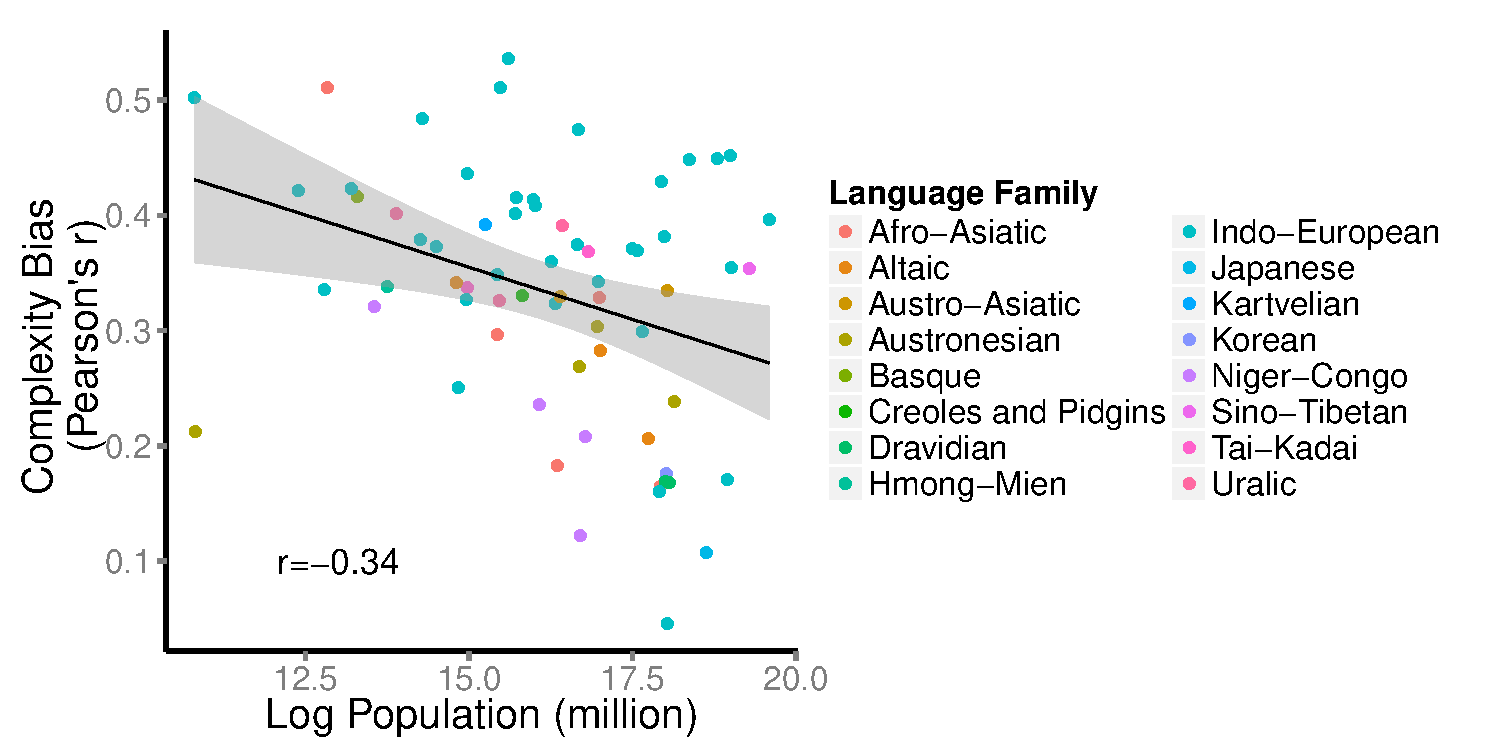
\includegraphics[width=3.2in]{Fig2.pdf}
%\caption{Relationship between complexity bias and speaker population. Each point corresponds to a language. \label{fig2}}
%\end{SCfigure}

These data reveal systematic cross-cultural variability in semantics, and suggest that  speakers' physical and linguistic proximity may contribute to convergence on shared semantics.

%The extent to which one person understands another when she says ``tree," then is determined in part by their shared cultural background, and 
\bibliographystyle{apacite}
\bibliography{evolang12} 

\end{document}
